\documentclass[output=paper]{langsci/langscibook} 
\ChapterDOI{10.5281/zenodo.2583818}
\author{Susanne Maria Michaelis\affiliation{Leipzig University \& Max Planck Institute for the Science of Human History (Jena)}}
\title{Support from creole languages for functional adaptation in grammar: Dependent and independent possessive {person}-forms}
\shorttitlerunninghead{Support from creole languages for functional adaptation in grammar}
\abstract{It seems to be a robust empirical observation that independent possessive\is{possessive construction} per\-son-forms (such as English \textit{mine, yours, hers}) are always longer than (or as long as) the corresponding adnominal possessive\is{possessive construction} per\-son-forms (such as English \textit{my, your, her}). Since adnominal forms are also much more frequent\is{frequency} in discourse than independent forms, this universal coding asymmetry can be subsumed under the grammatical form-frequency correspondence hypothesis \citep{HaspelmathEtAl2014}. In other words, the fact that independent possessive\is{possessive construction} forms are longer can be seen as a functional response to the need to highlight rarer, less predicatable\is{predictability} forms.\newline In this paper, I present evidence from creole languages and show that irrespectively of their young age and extremely accelerated grammaticalization processes, these high-contact languages confirm the coding asymmetry. Moreover, creole languages, just as non-creole languages, show a diverse array of diachronic pathways all leading eventually to longer independent possessive\is{possessive construction} per\-son-forms. Such a case of multi-convergence of structures through very different diachronic processes strongly suggests that the current patterns cannot be explained exclusively on the basis of the sources and the kinds of changes that commonly give rise to independent (and adnominal) possessive\is{possessive construction} forms, but that there is an overarching functional efficiency principle underlying these coding asymmetries\is{coding asymmetry}.
}

\usepackage{langsci-gb4e}
% %% hyphenation points for line breaks
%% Normally, automatic hyphenation in LaTeX is very good
%% If a word is mis-hyphenated, add it to this file
%%
%% add information to TeX file before \begin{document} with:
%% %% hyphenation points for line breaks
%% Normally, automatic hyphenation in LaTeX is very good
%% If a word is mis-hyphenated, add it to this file
%%
%% add information to TeX file before \begin{document} with:
%% %% hyphenation points for line breaks
%% Normally, automatic hyphenation in LaTeX is very good
%% If a word is mis-hyphenated, add it to this file
%%
%% add information to TeX file before \begin{document} with:
%% \include{localhyphenation}
\hyphenation{
affri-ca-te
affri-ca-tes
com-ple-ments
Haw-kins
broad-er
over-view
par-tic-u-lar
spe-cif-ic
adap-tive
lin-guis-ti-cal-ly
Hix-kar-yana
sour-ces
mark-er
ground-ed
evol-ved
Born-kessel-Schlesew-sky
}
\hyphenation{
affri-ca-te
affri-ca-tes
com-ple-ments
Haw-kins
broad-er
over-view
par-tic-u-lar
spe-cif-ic
adap-tive
lin-guis-ti-cal-ly
Hix-kar-yana
sour-ces
mark-er
ground-ed
evol-ved
Born-kessel-Schlesew-sky
}
\hyphenation{
affri-ca-te
affri-ca-tes
com-ple-ments
Haw-kins
broad-er
over-view
par-tic-u-lar
spe-cif-ic
adap-tive
lin-guis-ti-cal-ly
Hix-kar-yana
sour-ces
mark-er
ground-ed
evol-ved
Born-kessel-Schlesew-sky
}
\begin{document}
\maketitle \is{possessive construction}\is{person}




\section{Introduction}

Languages are functionally adapted\is{adaptation} to their users’ needs in a variety of ways. This can be seen in a range of different domains, such as (i) text genres, (ii) social structure and (iii) the ecological \isi{environment}. The \isi{genre} of informal, spontaneous face-to-face communication is reflected in grammatical features of loosely connected discourse with mainly coordinated\is{coordination} or juxtaposed\is{juxtaposition} sentences, many hesitation phenomena, overlapping utterances, and piecemeal structuring of information in accordance with online \isi{processing} needs, whereas text genres intended for formal, planned, out-of-context, written communication show densely integrated information, multiple syntactic \isi{embedding} strategies and therefore longer sentences, and greater syntagmatic variation (\citealt{KochOesterreicher2012} [1985]). Secondly, languages are adapted\is{adaptation} to the social structuring of their users, for instance to the percentage of second language speakers\is{acquisition} in a speech community: In a well-known study, \citet{LupyanDale2010} analyzed data from the \textit{World atlas of language structures} \citep{HaspelmathEtAl2005} and found that the greater the number of second language speakers\is{acquisition} in a speech community, the simpler are aspects of the morphology of the languages spoken by these communities. In a similar vein, \citet{BentzWinter2013} found that languages with many second language speakers\is{acquisition} tend to have fewer morphological \isi{case}s. And third, it has been shown that speakers adapt\is{adaptation} their languages to their ecological \isi{environment}s, for example by using whistled speech in distant communication to overcome the background noise of rural environments (\citealt{Meyer2005,Meyer2008}). 

In the present chapter, I will look at yet another instance of functionally adapt\-ed\is{adaptation} linguistic structures: \isi{efficiency}-based universal coding asymmetries\is{coding asymmetry} in grammar, also called form-\isi{frequency} correspondences (see \citealtv{chapters/haspelmath}). More specifically, I will discuss one specific universal \isi{coding asymmetry} resulting from asymmetric \isi{frequency} of use patterns in discourse: the difference between dependent and independent possessive\is{possessive construction} \isi{person}-forms. Independent \is{person}{per\-son}-forms such as \textit{mine}, \textit{yours}, \textit{hers}, and \textit{ours} are coded with forms that are longer than or equally long as dependent possessive \isi{person}-forms such as \textit{my, your, her,} and \textit{our}. I claim that the reason for this is a general \isi{efficiency} principle: Less frequent\is{frequency} and therefore more surprising\is{surprisal} meanings need more costly coding than more frequent\is{frequency} and therefore more predicatable\is{predictability} meanings. 

Such functional-adaptive\is{adaptation} explanations have a diachronic component \citep{Bybee1988}: Since the current system is often rigidly conventional, the adaptive\is{adaptation} forces must have been active in earlier diachronic change. But how can we understand such a development? Functionally adapted\is{adaptation} coding asymmetries\is{coding asymmetry}, as seen in dependent/independent possessive\is{possessive construction} \isi{person}-forms, are the outcome of hundreds, sometimes thousands of years of language change processes. These processes reflect countless speech acts between interlocutors adding up incrementally and resulting in the crystallization of functionally adapted\is{adaptation} grammatical structures over time. As grammatical change progresses at an extremely slow pace compared to other cultural \isi{evolution}ary processes, the step-by-step changes which bring about functionally adapted\is{adaptation} grammatical structures are often opaque or difficult to trace, even in languages with a well-documented written history (see \citealtv{chapters/serzant}). To circumnavigate this difficulty, I will focus on \isi{creole} languages, which are born out of extremely accelerated change processes in the context of the European colonial expansion, roughly during the 16\textsuperscript{th} to 20\textsuperscript{th} centuries. These high-\isi{contact} languages have evolved their complex grammatical structures within only a few hundred years. In this way they are a good test case for functional-adaptive\is{adaptation} change processes because \isi{creole}s demonstrate in a kind of fast motion what happens to grammatical structures under functional pressures, which in less contact-influenced languages would have taken hundreds (or thousands) of years to evolve. In this way, \isi{creole}s open a unique window on grammatical change processes which in these languages can be traced gradually from their transparent source constructions to various further grammaticalized\is{grammaticalization} stages, processes which are supposed to be operative in all languages at all times, but which take much more time to proceed in languages less heavily influenced by \isi{contact}. 

I make two main points in this paper:

(i) Evidence from \isi{creole} languages indeed confirms the \isi{coding asymmetry}: Independent \isi{person}-forms are coded with forms that are always longer than, or as long as, the dependent \isi{person}-forms, but never shorter.

(ii) Creole languages, just as non-\isi{creole} languages, show a diverse array of diachronic pathways all leading eventually to longer independent possessive\is{possessive construction} \isi{person}-forms. Such a case of multi-\isi{convergence} of structures through very different diachronic processes strongly suggests that there is an overarching functional \isi{efficiency} principle underlying these coding asymmetries\is{coding asymmetry} (see \citealtv{chapters/haspelmath}). 

After introducing the \isi{coding asymmetry} in possessive\is{possessive construction} \isi{person}-forms in \sectref{sec:michaelis:2}, in \sectref{sec:michaelis:3} I discuss various types of source constructions and diachronic pathways which lead to longer independent possessive\is{possessive construction} \isi{person}-forms. Then in \sectref{sec:michaelis:4}, I present a range of cases from \isi{creole} languages and their various diachronic pathways. In \sectref{sec:michaelis:5}, I consider but ultimately reject some alternative explanations against the background of the functional \isi{efficiency}-based explanation adopted in this article. 

\section{Coding asymmetry: Dependent vs. independent possessive {person}-forms}\label{sec:michaelis:2} \is{person}

Dependent possessive\is{possessive construction} per\-son-forms always occur together with an overt noun within a nominal phrase, as in \textit{your house}, whereas independent possessive\is{possessive construction} {per\-son}-forms occur without an overt noun, as in \textit{mine}. In the latter case, the referent of the noun is understood from the context because of an anaphoric\is{anaphora} relationship, as in (1a) and (1b), or because of a predicative use, as in (1c).  

%%1st subexample: change \ea\label{...} to \ea\label{...}\ea; remove \z  
%%further subexamples: change \ea to \ex; remove \z  
%%last subexample: change \z to \z\z 
\ea
\ili{English}
\ea
Your house is bigger than mine. (= ‘than my house’)
\ex
 Their dog is in a kennel, but ours sleeps under my bed. (= ‘our dog’)
\ex 
 Is this bike yours? (= ‘your bike’)
\z
\z

In a recent study, \citet{Ye2017}{\-}\footnote{\citet{Ye2017} analyzes a sample of 69 genealogically and areally unrelated languages.} has found that in the world's languages independent possessive\is{possessive construction} \isi{person}-forms like \ili{English} \textit{mine}, \ili{French} \textit{le mien} ‘mine’, and Mandarin \il{Chinese (Mandarin)} Chinese \textit{wo de} ‘mine’ are coded with forms that are longer than or equally long as the corresponding dependent possessive\is{possessive construction} \isi{person}-forms, such as \ili{English} \textit{my,} \ili{French} \textit{mon} ‘my’, or at least not shorter, as illustrated by Mandarin \il{Chinese (Mandarin)} Chinese \textit{wo de} ‘my’. Coding length here refers to the number of segments in the signal, or possibly to the amount of biomechanical effort (see \citealt{NapoliEtAl2014} with regard to \ili{sign language}s). Most importantly, examples of counter-asymmetric coding\is{coding asymmetry} are not attested, i.e. there are no languages where the dependent possessive\is{possessive construction} \isi{person}-forms are longer than independent possessive\is{possessive construction} \isi{person}-forms, e.g. *\textit{mine house} vs. \textit{my} ‘mine’. Note that (in)dependent possessive\is{possessive construction} \isi{person}-form can be manifested through a range of language-specific structures, also embracing complex forms, such as combinations of \isi{article}s or \isi{adposition}s with \isi{pronoun}s, as in \ili{French} \textit{le mien} and Mandarin \il{Chinese (Mandarin)} Chinese \textit{wo de} [I \textsc{gen}]. 

\largerpage
\tabref{tab:michaelis:1} shows a number of different types of correspondences between dependent and independent \isi{person}-forms in the world's languages: Firstly, many languages code the two types of \isi{person}-forms identically and thus with equally long forms, as for instance in Mandarin \il{Chinese (Mandarin)} Chinese. In other languages, the independent \isi{person}-form has an additional marker compared to the dependent form. This can be a substantivizer\is{nominalization}, as in \ili{Lezgian} (\textit{{}-di}), or an additional stem, as in \ili{Kanuri} (\textit{kaá}{}-). In some languages the definite\is{definiteness} \isi{article} is used to form the independent \isi{person}-form, such as in \ili{Italian} \textit{la mia} (with \isi{kinship} terms like \textit{sorella} ‘sister’).\footnote{If nouns like \textit{casa} ‘house’ or \textit{libro} ‘book’ were considered, \ili{Italian} would be classified just like Chinese \il{Chinese (Mandarin)} (identical pattern) because there would be no coding difference: \textit{la mia casa} ‘my house’ vs. \textit{la mia} ‘mine’, \textit{il mio libro} ‘my book’ vs. \textit{il mio} ‘mine’.} Yet another synchronic pattern in independent \isi{person}-forms consists in having extra material on the dependent form, as in \ili{Coptic} \textit{p-ô-k} [\textsc{art-indep-2sg}] ‘yours’ (vs. \textit{p-ek-ran} [\textsc{art-2sg}{}-name] ‘your name’).


\begin{table}
\small
\begin{tabularx}{\textwidth}{Qp{2cm}XXp{2cm}}
\lsptoprule

\bfseries Pattern type & \bfseries Language & \bfseries Dependent \isi{person}-form & \bfseries Independent \isi{person}-form & \bfseries Source\\
\midrule
identical & Mandarin \il{Chinese (Mandarin)} Chinese & \textit{wo}   \textit{de}  \textit{shu}


I   \textsc{gen}  book

‘my book’ & \textit{wo}  \textit{de~}

I  \textsc{gen}

‘mine’ & \\
\tablevspace

additional marker & \ilit{Lezgian} & \textit{zi}  \textit{ktab}

I.\textsc{gen}  book

‘my book’ & \textit{zi-di}

I.\textsc{gen-subst}

‘mine’ & \citet[110]{Haspelmath1993}\\

\tablevspace
additional stem & \ilit{Kanuri} & \textit{fewá-ndé}

cow-\textsc{1pl.poss}

‘our cows’ & \textit{kaá{}-nde}

\textsc{indep-1pl}

‘ours’ & \citet[31f.]{Cyffer1998_Kanuri}\\


\tablevspace
additional \isi{article}~ & \ilit{Italian} & \textit{mia sorella}

‘my sister’ & \textit{la mia}

‘mine’ & \citet[44,286f.]{Schwarze1988}\\


\tablevspace
longer form & \ilit{Coptic} & \textit{p-ek-ran}

\textsc{art-2sg}{}-name

‘your name’ & \textit{p-ô}\textit{{}-k}

\textsc{art-indep-2sg}

‘yours’ & \citet[277]{Haspelmath2015}\\
\lspbottomrule
\end{tabularx}

\caption{Some types of correspondences of dependent and independent per\-son-forms}
\label{tab:michaelis:1}
\end{table}

Apparently the only possible generalization which can be drawn from the typological variation is that the independent \isi{person}-form is always longer than, or as long as, the dependent \isi{person}-form, but never shorter\footnote{See also \citet{Croft1991}, who very similarly predicts “function-indicating morphosyntax” in all the atypical combinations of lexical semantic class and pragmatic\is{pragmatics} functions, whereas typical combinations lack function-indicating markers \citep[51]{Croft1991_Cat}), e.g. marked predicative nominals vs. unmarked\is{zero marking} nouns, or marked predicative adjectives\is{adjective} vs. unmarked\is{zero marking} attributive adjectives.}.

Now the claim is that these coding asymmetries\is{coding asymmetry} reflect asymmetries of \isi{frequency} of use. More frequent\is{frequency} meanings (here: dependent possessives) are more predicatable\is{predictability} and therefore speakers or signers can reduce the amount of the linguistic signal in taking into account how much of the signal hearers and receivers (in sign languages) need in order to successfully reconstruct the intended meaning. By contrast, less frequent\is{frequency} meanings (here: independent possessives\is{possessive construction}) are in need of a greater amount of signal coding for the hearer to be able to infer\is{inference} the meaning. 

Indeed, \isi{frequency} counts of three large text corpora\is{corpus} of three different languages (\ili{English}, \ili{Korean}, and Mandarin \il{Chinese (Mandarin)} Chinese\footnote{For \isi{frequency} counts in \ili{Korean} and Mandarin \il{Chinese (Mandarin)} Chinese, see \citealt{Ye2017}.}) confirm the hypothesis that dependent and independent \isi{person}-forms are unequally spread over discourse in such a way that dependent possessive\is{possessive construction} \isi{person}-forms are generally more frequent\is{frequency} than their independent counterparts. \tabref{tab:michaelis:2} shows data from British \ili{English}.

\begin{table}
\begin{tabularx}{\textwidth}{Xr@{\qquad\qquad}Xr}
\lsptoprule

\bfseries Dependent & \bfseries Token \isi{frequency} & \bfseries Independent & \bfseries Token \isi{frequency}\\
\midrule
\textit{my} & 145,250 & \textit{mine} & 6,067\\
\textit{your} & 132,598 & \textit{yours} & 4,059\\
\textit{our} & 92,314 & \textit{ours} & 1,658\\
\textit{their} & 251,410 & \textit{theirs} & 976\\
\lspbottomrule
\end{tabularx}

\caption{(In)dependent possessive per\-son-forms in the British National Corpus\is{corpus}}
\label{tab:michaelis:2}
\end{table}

Interestingly, \isi{frequency} counts from Mandarin \il{Chinese (Mandarin)} Chinese, a language without a \isi{coding asymmetry} in possessive\is{possessive construction} \isi{person}-forms, give the same results as counts for \ili{English} and \ili{Korean}, which have the \isi{coding asymmetry} in possessive\is{possessive construction} \isi{person}-forms (see \citealt{Ye2017}). Therefore, the prediction is that we find similar \isi{frequency} distributions of dependent and independent possessive\is{possessive construction} \isi{person}-forms in all languages, independently of whether the universal \isi{coding asymmetry} is grammaticalized\is{grammaticalization} or not.

\section{Types of source constructions and diachronic pathways}\label{sec:michaelis:3}

As noted earlier, synchronic universal coding asymmetries\is{coding asymmetry} have a diachronic correlate because the adaptive\is{adaptation} forces must have been active in earlier stages of the language and have kept shaping grammatical structures according to the functionally motivated \isi{efficiency} principle: less predicatable\is{predictability} meanings need more coding and more predicatable\is{predictability} meanings need less coding.

There is a wide variety of sources and diachronic pathways by which independent possessive\is{possessive construction} \isi{person}-forms come to be longer than the dependent forms. Generally, one can distinguish two scenarios: either the more frequent\is{frequency} member of the grammatical opposition is shortened \citep{Bybee2007}, or the rarer member of the grammatical opposition is lengthened\footnote{Here, the term ‘lengthening’ mainly refers to processes by which a given linguistic form is expanded or augmented by new lexical or morphosyntactic material. But – in principle –~lengthening may also pertain to phonological/phonetic processes, such as vowel lengthening or \isi{gemination}.} \citep{Haspelmath2008_Econ}. In the shortening scenario, speakers assess what hearers can predict and adjust their articulations accordingly, resulting in shortening\is{phonetic reduction} of the signal of the more frequent\is{frequency} form of a grammatical opposition. In this way, Old \ili{English} \textit{min} ‘my’ was eventually shortenend to Modern \ili{English} \textit{my}, likewise Old \ili{Spanish} \textit{mío} was shortened to Modern \ili{Spanish} \textit{mi}. The \ili{Coptic} contrast between \textit{pôk} ‘yours’ and \textit{pek} ‘your’ that we saw in \tabref{tab:michaelis:1} is likewise attributable to shortening of the earlier full \isi{person}-form \textit{pôk} to \textit{pek-}. The shortened form became a dependent \isi{person}-form whereas the old from \textit{pôk} became restricted to the independent function (Eitan \iai{Grossman} p.c.).

The lengthening scenario can be described as follows: When hearers are in danger of making wrong predictions\is{predictability}, speakers tend to help them by using forms which – compared to the rarer\is{frequency} member of the opposition – have been lengthened with some extra material. One example comes from \ili{German}, where the independent form \textit{der mein-ig-e} [\textsc{def} \textsc{1sg.poss-indep-masc.sg.nom}] ‘mine’ is based on the dependent form \textit{mein} ‘my’ plus an additional suffx \textit{{}-ig,} which occurs in other derived \isi{adjective}s (like \textit{selb-ig} ‘same’, \textit{bärt-ig} ‘bearded’, \textit{ehrgeiz-ig} ‘ambitious’). As we see in Tables \ref{tab:michaelis:3a} and \ref{tab:michaelis:3b}, the array of source constructions and diachronic pathways which give rise to longer independent possessive\is{possessive construction} \isi{person}-forms is very diverse.

\begin{table}
\small
\begin{tabularx}{\textwidth}{lQll}
\lsptoprule
\bfseries Language & \bfseries Strategy & \bfseries Dependent form & \bfseries Independent form\\
\midrule
\ili{English} & phonological reduction\is{phonetic reduction} of dependent form &  \textit{my} & \textit{mine}\\
\lspbottomrule
\end{tabularx}
\caption{Shortened dependent form}
\label{tab:michaelis:3a}
\end{table} 

\begin{table}
\begin{tabularx}{\textwidth}{Q@{}>{\raggedright}p{30mm}p{20mm}Q}
\lsptoprule
\bfseries Language & \bfseries Strategy & {\bfseries Dependent form} & \bfseries Independent form\\
\midrule 
\ilit{German} & {affixal lengthening} & \textit{mein} \newline[\textsc{1sg.poss}] & \textit{der mein-ige} \newline\mbox{[\textsc{def} \textsc{1sg.poss-indep}]}\\
\tablevspace
\ilit{Arabic} & dummy noun: ‘property’ & {\textit{{}-ii}{\textit{~} }\newline[\textsc{1sg.poss}]} & \textit{milk-ii} {\textit{~}}\newline[property-\textsc{1sg.poss}] {~ ~ ~}\\
\tablevspace
\ilit{Greek} & \mbox{intensified \isi{person}} form ‘own’ & {\textit{mu} \newline[\textsc{1sg.poss}]} & \textit{dhikó mu} \newline[\textsc{intens} \textsc{1sg.poss}]      \\
\tablevspace
\ilit{Diu Indo-Portuguese} & use of \mbox{\isi{adposition} ‘of, for’} & {\textit{mi}  \newline[\textsc{1sg.poss}]} & \textit{də mi} \newline[of \textsc{1sg.poss}]  \\
\tablevspace
\ilit{Albanian} & use of definite\is{definiteness} \isi{article} & {\textit{im} \newline[\textsc{1sg.poss}]} & \textit{im-i}  \newline[\textsc{1sg.poss-def}]\\
\tablevspace
\ilit{Berbice Dutch} & general nominalizer\is{nominalization} & {\textit{ɛk}\textit{ɛ} \newline[\textsc{1sg.poss],} \textsc{\newline[1sg]}}  & \textit{ɛk}\textit{ɛ{}-j}\textit{ɛ} \newline[\textsc{1sg.poss-nmlz]}    \\

\tablevspace
\ilit{English} (dialectal) & \isit{exaptation} & {\textit{her} \newline[\textsc{3sg.F.poss}]}  & \textit{her-n} \newline[\textsc{3sg.poss-indep}]  \\
\lspbottomrule
\end{tabularx}
\caption{Lengthened independent form}
\label{tab:michaelis:3b} 
\end{table}


The different strategies range from the use of a dummy noun (‘my thing’, ‘my property’), intensified \isi{person} forms (‘my own’), the use of \isi{adposition}s (‘of my’) and definite\is{definiteness} \isi{article}s (‘the my’) to general nominalizer\is{nominalization} (‘my one’). One special strategy to arrive at longer independent possessive\is{possessive construction} \isi{person}-forms consists in recruiting already existing pronominal\is{pronoun} (lengthened) forms which have been used for other grammatical functions. One example comes from Middle \ili{English} varieties, where the independent possessive\is{possessive construction} forms \textit{her-n, our-n, their-n} (still surviving in \ili{English} dialects today, see \citealt{KortmannLunkenheimer2013}) go back to erstwhile feminine \isi{dative} \isi{case}-marked pronominal\is{pronoun} forms with the suffix \textit{{}-n} (\textit{hire-n} [\textsc{3sg.fem.dat}] ‘to her’). In Middle \ili{English}, such \isi{dative} forms got re-used, or “exapted”\is{exaptation}, to function as independent possessive\is{possessive construction} forms, also under the additional analogical\is{analogy} pressure from the \textit{my/mine} and \textit{thy/thine} oppositions (see \citealt{Allen2002}, and for the notion of \isi{exaptation}, see \citealt{Lass1990,Lass2017,NordeVandeVelde2016} and the discussion below). 

Irrespectively of the shortening or the lengthening scenario, \textsc{all} these developments result in coding asymmetries\is{coding asymmetry} which work in the \textsc{same} direction: The less frequent\is{frequency} member (here the independent possessive\is{possessive construction} \isi{person}-form) is coded with a form that is always coded as least as long as the more frequent\is{frequency} member of the pair, but never shorter.

\newpage 
Now how do \isi{creole} languages fit into this picture? In the next section, I will consider possessive\is{possessive construction} \isi{person}-forms in various \isi{creole} languages from around the world (based on the \textit{Atlas of \isi{pidgin} and \isi{creole} language structures}, \citealt{MichaelisEtAl2013}, apics-online.info) to check whether the universal trend identified by typological work can be supported by these high-\isi{contact} languages.


\section{Diverse pathways in {creole}s}\label{sec:michaelis:4}
\is{creole}

Before looking at possessive\is{possessive construction} \isi{person}-forms in \isi{creole} languages, I would like to highlight one characteristic feature of these languages which is crucial for the argument put forward in this paper: Creole\is{creole} languages show an unusual amount of freshly grammaticalized\is{grammaticalization} material due to an accelerated pace of grammatical change processes (\citealt{HaspelmathMichaelis2017}; \citealt{MichaelisHaspelmath2018}). Examples come from \isi{tense}-\isi{aspect}-\isi{mood} markers, such as the \ili{Negerhollands} \isi{future} \isi{tense} marker \textit{lo} < \textit{loo} ‘go’ < \ili{Dutch} \textit{lopen} ‘run’, or the \ili{Jamaican} \isi{anterior} marker \textit{wehn} < \ili{English} \textit{been}. Creoles\is{creole} also show newly grammaticalized\is{grammaticalization} \isi{case} markers, such as the \isi{dative} marker \textit{pe} in \ili{Diu Indo-Portuguese} (< \ili{Portuguese} \textit{para}), the \isi{accusative} marker \textit{ku} in \ili{Papiá Kristang} (< \ili{Portuguese} \textit{com} ‘with’), or \isi{voice} markers, such as the \isi{reciprocal} marker \textit{kanmarad} in \ili{Seychelles Creole} (< \ili{French} \textit{camarade}). The explanation for these widespread newly grammaticalized\is{grammaticalization} markers appears to be as follows: Speakers communicating in high-\isi{contact} situations which involve many second language speakers\is{acquisition} tend to rely on extra \isi{transparency} of their utterances in order to successfully get their messages across.\footnote{See already \citet{SeurenWekker1986} for the notion of \isi{transparency} in the creolization process.} These instances of extra \isi{transparency} give rise to newly grammaticalized\is{grammaticalization} structures by refunctionalizing erstwhile content words or otherwise less grammaticalized\is{grammaticalization} constructions, as seen in the examples cited above.

Turning to possessive\is{possessive construction} forms, let us now consider the following three guiding questions: 
\begin{itemize}
\item Do \isi{creole}s confirm the universal \isi{coding asymmetry} discussed in this paper?
\item Does the need for extra \isi{transparency} translate into freshly grammaticalized\is{grammaticalization} constructions also in the domain of possessive\is{possessive construction} \isi{person}-forms?
\item Which kinds of source constructions give rise to the various possessive\is{possessive construction} \isi{person}-forms?
\end{itemize}

The answer to the first question is a straightforward yes: The \isi{creole} evidence, which comes from 59 \isi{creole}s world-wide with different lexifier and substrate languages (see \citealt{HaspelmathApics2013} and \figref{fig:michaelis:1} in the Appendix), confirm the universal \isi{coding asymmetry}: Independent possessive\is{possessive construction} \isi{person}-forms are coded with forms that are longer than or equally long as dependent possessive\is{possessive construction} \isi{person}-forms. Some examples are given in \tabref{tab:michaelis:4}. 

\begin{table}
\begin{tabularx}{\textwidth}{XXX}
\lsptoprule

\bfseries Creole\is{creole} language & \bfseries Dependent form & \bfseries Independent form\\
\midrule

\ilit{Bislama}


\citep{Meyerhoff2013} & \textit{blong yu}{\textit{~}}

[\textsc{poss} \textsc{2sg}] ‘your’ & \textit{blong yu}{\textit{~}} {\textit{~ ~ ~ ~ ~ ~ ~ ~ ~ ~ ~ ~ ~}}

[\textsc{poss} \textsc{2sg}] { ‘}yours’\\

\tablevspace

\ilit{Kinubi}


\citep{Luffin2013} & \textit{tá-i}

[\textsc{poss-1sg}] ‘my’ & \textit{tá-i}

[\textsc{poss-1sg}] ‘mine’\\

\tablevspace

\ilit{Batavia Creole} 


\citep{Maurer2013} & \textit{minya} 

[\textsc{1sg.poss}] ‘my’ & \textit{minya}\textbf{ }\textit{sua}\textbf{ }

[\textsc{1sg.poss} \textsc{poss}] ‘mine’\\

\tablevspace

\ilit{Martinican Creole}


(\citealt{ColotLudwig2013}) & \textit{{}-mwen}

[\textsc{1sg.poss}] ‘my’ & \textit{ta mwen}

[\textsc{poss} \textsc{1sg.poss}] ‘mine’\\

\tablevspace

\ilit{Pichi}


\citep{Yakpo2013} & \textit{yù} {\textit{~}}

[\textsc{2sg.poss}], [2sg] ‘you’ & \textit{yù yon}

[\textsc{2sg.poss} own] ‘yours’\\

\tablevspace

\ilit{Palenquero}


\citep{Schwegler2013} & \textit{mi}

[\textsc{1sg.poss}] ‘my’ & \textit{ri mi}

[of \textsc{1sg.poss}] ‘mine’\\
\lspbottomrule
\end{tabularx}

\caption{Dependent and independent possessive per\-son-forms in some creole languages}
\label{tab:michaelis:4}
\end{table}

\noindent The following \tabref{tab:michaelis:5} presents a quantitative overview of the different construction types found in \isi{creole} languages of \textit{APiCS}. Here, only languages with an exclusive value assignment are considered (48 out of 59 \isi{creole} languages).

\begin{table}
\begin{tabularx}{\textwidth}{l>{\raggedright}p{5.5cm}Y}
\lsptoprule

\bfseries Coding pattern & \bfseries Feature value & \bfseries Number of \isi{creole} languages in \textit{APiCS}\\
\midrule
Symmetry & Identical to dependent pronominal\is{pronoun} possessor & 20\\

\tablevspace
Asymmetry & Special \isi{adposition} plus \isi{pronoun} & 9\\
\tablevspace
 & Other word plus dependent pronominal\is{pronoun} possessor & 13\\
\tablevspace
 & Special form for independent pronominal\is{pronoun} possessor & 6\\
\midrule
& Total & 48\\
\lspbottomrule
\end{tabularx}

\caption{Distribution of different construction types over 48 creoles in independent possessive per\-son-forms (\textit{APiCS} Feature 39)}
\label{tab:michaelis:5}
\end{table}

Likewise, the answer to the second question raised above is positive: The majority of the possessive\is{possessive construction} \isi{person}-forms are indeed freshly grammaticalized\is{grammaticalization} and therefore still transparent enough to be traced quite closely with respect to the different diachronic processes that have brought about their \isi{coding asymmetry}. 
\newpage
Coding asymmetries\is{coding asymmetry} explicitly allow for the two forms of an opposition to be equally long (either overtly or zero-coded\is{zero marking})\footnote{See also \citet[58f.]{Croft1991}, who calls such cases \textsc{neutral} evidence.}, as is the case in Mandarin \il{Chinese (Mandarin)} Chinese \textit{wo de} ‘my’, ‘mine’ cited above. As \tabref{tab:michaelis:5} shows, there are quite a number of \isi{creole} languages which show this coding pattern, i.e. no length difference in the coding of both forms, as for instance in \ili{Tok Pisin} \textit{bilong mi} [\textsc{poss} \textsc{1sg}] ‘my’, ‘mine’ or the related language \ili{Bislama} (see \tabref{tab:michaelis:4}). These languages do not contradict the universal \isi{coding asymmetry}, as they do not show the opposite coding pattern, i.e. longer dependent forms against shorter independent forms.

Let us now turn to \isi{creole} languages for which we can attest a \isi{coding asymmetry} in possessive\is{possessive construction} forms. As for the source constructions, I will first look at cases of shortening that parallel the \ili{English} development from \textit{mine to my}. One example comes from Juba Arabic \il{Arabic (Juba)}, where the original form \textit{bita-i} [\textsc{poss-1sg}] ‘my/mine’ gets shortened and at some point reanalyzed\is{reanalysis} as the dependent possessive\is{possessive construction} \textit{tá-i} ‘my’, as in \textit{ída tái} [hand \textsc{1sg.poss}] ‘my hand’ (\citealt{ManfrediPetrollino2013}), whereas the older non-shortened form \textit{bita-i} continues to be used as the independent possessive\is{possessive construction} form meaning ‘mine’. 

However, the vast majority of asymmetric correspondence types in \isi{creole} languages – as in non-\isi{creole} languages – follow the second scenario described in \sectref{sec:michaelis:3}: the \isi{coding asymmetry} comes about by some process of expanding the less frequent\is{frequency} member of the grammatical opposition. One widespread source is the use of an \isi{adposition} going back to ‘of’ or ‘for’ in one of the European lexifier languages \ili{French}, \ili{Portuguese}, \ili{English} etc. An example comes from \ili{Portuguese}-based \ili{Santome} \citep{Hagemeijer2013}, where the dependent possessive\is{possessive construction} \isi{person}-form \textit{mu} ‘my’, which is expanded by the \isi{genitive} \isi{preposition} \textit{ji} (< \ili{Portuguese} \textit{de} ‘of’), gives rise to the independent possessive\is{possessive construction} form \textit{ji mu} ‘mine’. \ili{Jamaican} \textit{fi-mi} ‘mine’ is another instance of the lengthening of the dependent form \textit{mi} \textsc{‘1sg.poss’} (and also 1\textsc{sg} ‘I’) by the \isi{preposition} \textit{fi} ‘for’ (< \ili{English} \textit{for}).

A second source construction for independent possessive\is{possessive construction} \isi{person}-forms in \isi{creole} languages involves the use of a dummy noun, such as ‘part’ or ‘thing’ (as mentioned above), as in \ili{Haitian Creole} \textit{pa m nan} [part \textsc{1sg.poss} \textsc{def}] ‘mine’ (lit. ‘my part’, \textit{pa} < \ili{French} \textit{part} ‘part’) as opposed to dependent forms, such as -\textit{m} (\textit{nan}) [\textsc{1sg.poss} \textsc{(def)]} ‘my’ in \textit{se m} [sister \textsc{poss.1sg]} ‘my sister’. The polysemous morpheme \textit{pa}, which in some contexts still has the original lexical meaning ‘part’, has grammaticalized\is{grammaticalization} into a possessive\is{possessive construction} form which can also be used in contexts where the possessor is stressed, as in (2).

\ea
{\ili{Haitian Creole} \citep{Fattier2013}  }\\
\gll Liv  pa  m    nan  bèl.\\
     book  \textsc{poss}  \textsc{poss.1sg} \textsc{def}  beautiful \\
\glt ‘MY book is beautiful.’
\z

\noindent However, the non-stressed noun phrase would be \textit{liv m} [book \textsc{poss.1sg]} ‘my book’ \citep{Fattier2013}. Here, we clearly see that the postposed morpheme \textit{pa} in \textit{pa m} does not denote a part of something, but has grammaticalized\is{grammaticalization} into a possessive\is{possessive construction} marker, as the literal meaning ‘book my part’ is not available for this construction. The same holds for the independent possessive\is{possessive construction} form \textit{pa m nan} ‘mine’: the meaning is not ‘my this part’, but \textit{pa} has become part of the newly grammaticalized\is{grammaticalization} independent possessive\is{possessive construction} form ‘mine’. 

A third source construction for independent possessive\is{possessive construction} forms features an \isi{intensifier} which is added to the dependent possessive\is{possessive construction}, as in \ili{Krio} \textit{mi yon} [\textsc{1sg.poss} \textsc{intens.own}] ‘mine’ (the dependent possessive\is{possessive construction} form being \textit{mi} ‘my’) \citep{Finney2013}.

There is a fourth source of independent forms involving a general (adjectival\is{adjective}) nominalizer\is{nominalization}, such as ‘one’. In \ili{Berbice Dutch}, there is a general nominalizer\is{nominalization} \textit{{}-jɛ} which is added to the personal \isi{pronoun} \textit{ɛkɛ} [\textsc{1sg.poss}]/[1\textsc{sg}] ‘my’ (‘I’), resulting in \textit{ɛkɛ-jɛ} [\textsc{1sg.poss-nmlz}] ‘mine’ (see \tabref{tab:michaelis:3b}). This nominalizer\is{nominalization} goes back to Eastern \ili{Ijo}, the substrate language of \ili{Berbice Dutch}, where it has \isi{singular} nonhuman reference, whereas in \ili{Berbice Dutch} it has grammaticalized\is{grammaticalization} into a generic nominalizer\is{nominalization} \citep{Kouwenberg2013}.

A fifth source can be illustrated with an example from \ili{Reunion Creole}, where the  \isi{determiner}/\isi{demonstrative} \textit{sa} is one of the lengthening elements (besides the \isi{genitive} \isi{preposition} \textit{d}) in the independent possessive\is{possessive construction} \isi{person}-form \textit{sa d mwen} [\textsc{dem} of \textsc{1sg}] ‘mine’, compared to the dependent form \textit{mon} [\textsc{1sg.poss}] ‘my’.

In some \isi{creole} languages the source construction is not known, as in \ili{Louisiana Creole}. Here, the marker \textit{kenn} is used as a morpheme to code the independent possessive\is{possessive construction} \isi{person}-forms, as in \textit{mo-kenn} [\textsc{1sg.poss-poss}] ‘mine’. This morpheme could perhaps be traced back to a \textsc{2sg.fem} independent \isi{person}-form in \ili{French} \textit{tienne} ‘yours’, which has developed into /kien/, which would then have analogically\is{analogy} spread to the whole paradigm, as in \textit{mo-kenn} [\textsc{1sg.poss-poss}] ‘mine’, \textit{to-kenn} [\textsc{2sg.poss-poss}] ‘yours’, \textit{li-kenn} [\textsc{1sg.poss-poss}] ‘his’ (\citealt{Neumann-HolzschuhKlingler2013}, Neumann-Holzschuh p.c.). The unusual feature in this scenario is the idea that it is the second-\isi{person} form which analogically\is{analogy} spreads to all other \isi{person}s, and not the more frequent\is{frequency} \textsc{1sg} or \textsc{3sg} forms. Whether this is the right \isi{reconstruction} of the origin of \textit{kenn} is not clear.

Generalizing over all instances of newly grammaticalized\is{grammaticalization} independent possessive\is{possessive construction} forms in \isi{creole} languages, we can state that irrespectively of the diverse source constructions, it is the independent possessive\is{possessive construction} \isi{person}-form that, in \textsc{all} instances, is longer than, or as long as, the dependent \isi{person}-form, but never shorter.


\section{Possible alternative explanations}\label{sec:michaelis:5}

We have seen that the cross-\isi{creole} data support the universal \isi{coding asymmetry} in possessive\is{possessive construction} \isi{person}-forms, and that this synchronic asymmetry can be explained by a functional-adaptive\is{adaptation} constraint of coding \isi{efficiency}: More frequent\is{frequency}ly expressed meanings (dependent possessive\is{possessive construction}s) need less costly signal encoding because they are highly predicatable\is{predictability}, whereas less frequent\is{frequency}ly expressed meanings need more robust signal encoding because they are less predicatable\is{predictability} (\citealtv{chapters/haspelmath}; see \citealt{NorcliffeJaeger2016} and \citealt{JaegerBuz2018} for supporting \isi{psycholinguistic} evidence in other domains of morphosyntax). Before concluding this paper, I will consider several alternative explanations, but reject them all as less convincing.


\subsection{Semantics, iconicity, and syntax}

Some functional linguists might argue for an alternative, semantically based or \isi{iconicity}-based explanation here, namely that the independent possessive\is{possessive construction} form is semantically more complex\is{complexity} in that it combines possession and referentiality, and so additional material has to be adduced in order to express this more complex concept, or to compensate for the absence of an overt nominal. 

\largerpage
But I would reject such a proposal because it is not obvious that independent possessors are semantically more complex. Rather, we can think of the situation as follows: Possessors refer to objects and persons, but at the same time, when used in \isi{possessive construction}s, they also express properties, like \isi{adjective}s. In the most frequent\is{frequency} use, possessive\is{possessive construction} forms (again like \isi{adjective}s) have a modification\is{modifier} function, as in \textit{my house} (the “unmarked\is{markedness}” use in terms of \citealt{Croft1991}). But when possessive\is{possessive construction} forms are used in the less frequent\is{frequency} referential function, as in \textit{mine}, specific marking is needed to highlight this unusual noun-like usage. Semantically, there is not really any difference in \isi{complexity} of both kinds of \isi{person}-forms: dependent possessive\is{possessive construction} forms combine \isi{person} and property with regard to possession in a \textsc{modification}\is{modifier} function, whereas independent \isi{person}-forms combine \isi{person} and property with regard to possession in a \textsc{reference} function. There is thus only a difference in the propositional function in which the semantic concepts are expressed (modification\is{modifier} vs. reference), but there is no \textsc{additional} semantic \isi{complexity} in independent possessive\is{possessive construction} \isi{person}-forms. 


Likewise, some linguists might argue that the motivation for the \isi{coding asymmetry} is purely syntactic, as the two possessive\is{possessive construction} forms occupy different syntactic slots. As the \isi{modifier}, such as \ili{French} \textit{mon}, cannot occur as the head of a NP, it has to be transformed into a noun by what \citet[58f.]{Croft1991_Cat} calls “function-indicating markers”, thus yielding \textit{le mien} ‘mine’ in \ili{French}. The use of the definite\is{definiteness} \isi{article} represents one of the lengthening processes in independent possessive\is{possessive construction} \isi{person}-forms that I described above. But I would interpret the mere use of function-indicating markers as the frozen grammaticalized\is{grammaticalization} results of hundreds or thousands of years of speakers performing communicatively efficient\is{efficiency} speech acts by marking the less predicatable\is{predictability} meanings with more elaborate linguistic matter. In this respect, there is no contradiction between today’s syntax and yesterday’s (and earlier) speakers' preferences to highlight less predicatable\is{predictability} meanings by more morphosyntactic material, which accumulated over generations and eventually contributes to the shaping of syntactic categories (see \citealt[171]{NorcliffeJaeger2016}\footnote{“Communicative \isi{efficiency} therefore holds explanatory potential not just for patterns of real-time language use, but also for the shape of grammars” (\citealt[171]{NorcliffeJaeger2016}.}). 


\subsection{ Diachronic change as a possible explanatory factor}

Yet a different type of explanatory account might propose that the diachronic origins of the relevant patterns give rise to the observed cross-linguistic distributions (see \citealt{Cristofaro2017}, and \citealtv{chapters/cristofaro}). The claim would be that the kinds of sources and diachronic pathways that bring about the observed patterns are tightly constrained (\isi{mutation}al constraints, see \citealtv{chapters/haspelmath}) and, crucially, that the \isi{coding asymmetry} is a direct but incidental result of how independent possessive\is{possessive construction} \isi{person}-forms emerge from their respective sources. 

The strongest argument against such a possible claim, and for an interpretation of the data in terms of a functional-adaptive\is{adaptation}, result-oriented approach, is the fact that we see \isi{convergence} of multiple sources and pathways toward a \textsc{uniform} outcome. In particular, the asymmetric coding\is{coding asymmetry} can come about through shortening or through lengthening. If there were no overarching functional constraint, we would expect many more counter-examples\is{exception} in the data, i.e. cases where the dependent possessive\is{possessive construction} \isi{person}-forms are longer than the independent ones, such as dependent *\textit{mine book} vs. independent *\textit{my} ‘mine’, or \ili{German} dependent *\textit{mein-iges Buch} ‘my book’ vs. independent *\textit{mein} ‘mine’, or \ili{Jamaican} dependent *\textit{fi-mi buk} ‘my book’ vs. independent *\textit{mi} ‘mine’. But this is not what we find.

The \isi{creole} data make clear that there is a surprisingly large array of source constructions which enter the pool of possible dependent and independent possessive\is{possessive construction}s. Many of these source constructions had different communicative functions when they were first grammaticalized\is{grammaticalization}. The use of a dummy noun ‘part’, for instance, which is the source of current \ili{Haitian Creole} independent possessive\is{possessive construction} \textit{pa m nan} ‘mine’, may have started out as a predicative \isi{focus} construction, such as ‘this is MY part’. This focussing function is still present in constructions like in example (2). But at some point, the morpheme \textit{pa} got refunctionalized into the phrase \textit{pa m nan}, which eventually got grammaticalized\is{grammaticalization} into the independent possessive\is{possessive construction} \isi{person}-form ‘mine’. How did this happen? I assume that speakers must have somehow felt that they needed a more elaborate, more fully marked form to convey to hearers that a less predicatable\is{predictability} meaning (independent possessive\is{possessive construction}) was expressed. Therefore they chose (elements of) an already existing construction, here the \isi{focus} construction, and through a kind of inflationary overuse grammaticalized\is{grammaticalization} it into the independent possessive\is{possessive construction} form \textit{pa m nan}, where the morpheme \textit{pa} does not have the meaning ‘part’ anymore. It is only at this moment that speakers created a grammatical opposition between a dependent and an independent possessive\is{possessive construction} form. 

\newpage 
Another source of a longer independent possessive\is{possessive construction} \isi{person}-form is the use of a \isi{preposition} ‘of/for’ together with a possessive\is{possessive construction} \isi{person} form ‘my/I’, yielding complex forms, such as ‘of my’ or ‘for me’, as seen in the \ili{Jamaican} independent possessive\is{possessive construction} form \textit{fi-mi} ‘mine’ (vs. dependent possessive\is{possessive construction} \textit{mi} [\textsc{1sg.poss]} ‘my’/[1\textsc{sg]} ‘I’, already cited above). Forms like \textit{fi-mi} may go back to a kind of predicative construction, such as ‘this is for me/this is of my’. But here again, at some point in time, the creators of \ili{Jamaican} refunctionalized the chunk \textit{fi-mi} to fit the need to highlight the more unusual, less predicatable\is{predictability} independent possessive\is{possessive construction} meaning ‘mine’. 


In this context, another fact makes a source-oriented account less convincing. Quite a few \isi{creole} languages show lengthened forms, such as \textit{fi-mi}, not only in the independent, but also in the dependent possessive\is{possessive construction} \isi{person}-form, as for instance in \ili{Zamboanga Chabacano} \textit{dimíyo} (‘of.1\textsc{sg}’) ‘my/mine’ or in \ili{Tok Pisin} \textit{bilong mi} (of.1\textsc{sg}) ‘my/mine’. This is the situation where there is no length difference in both forms, as illustrated for Mandarin \il{Chinese (Mandarin)} Chinese in \sectref{sec:michaelis:2} (identical pattern in \tabref{tab:michaelis:1}). If a hypothesized predicative construction were the source of the independent possessive\is{possessive construction} \isi{person}-forms, it certainly cannot be the source for the dependent form. Therefore, here we must allow for some kind of analogical extension\is{analogy} to the dependent forms. Interestingly, it is only in the dependent possessive\is{possessive construction} function that \textit{dimíyo} can be shortened to \textit{mí} \citep{Steinkrüger2013}, thus again giving rise to a new \isi{coding asymmetry} in the predicted direction: the independent possessive\is{possessive construction} form \textit{dimíyo} ‘mine’ is longer than the dependent possessive\is{possessive construction} form \textit{mí} (similar to \ili{English} \textit{mine/my} and Juba Arabic\il{Arabic (Juba)} \textit{bitai/tái}).

Coming back to both lengthening scenarios of independent possessive\is{possessive construction} forms described above: The crucial point here is the fact that the change process from a \isi{focus} or predicative construction to an independent possessive\is{possessive construction} form should not be seen as a self-propelling \isi{grammaticalization} process, but as a result of speakers' unconscious choices to communicate efficiently\is{efficiency} by highlighting the less predicatable\is{predictability} meaning, thus ultimately bringing about functionally adapted\is{adaptation} linguistic structures. In other words: If speakers did not sense the communicative need to mark independent possessive\is{possessive construction}s with more linguistic material, they would not drag parts of a \isi{focus} or predicative construction into an emergent independent possessive\is{possessive construction} \isi{person}-form in the first place. 

Therefore, speaking of \textsc{synchronic} “lengthening” strategies in independent possessive\is{possessive construction} forms, as I have done in the previous sections, could be misinterpreted. What generations of speakers really do while communicating is recruiting \textsc{already} \textsc{existing} structures (lexical or grammatical) to fit new grammatical functions (parts of old \isi{focus} constructions and old predicative constructions are used to express new independent possessive\is{possessive construction} forms). Linguists subscribing to the source-oriented approach would probably completely agree with this statement. But, as I laid out in the preceding paragraph, there is a second part to this story, where mere \isi{persistence} accounts fail to explain the data: While recruiting existing structures for new grammatical functions, speakers unconsciously comply with the \isi{efficiency} principle. As a result of the cumulative individual speech acts, we observe ever changing functionally adapted\is{adaptation} structures, which overwhelmingly point into the \textsc{same} direction: rarer, less predicatable\is{predictability} meanings tend to be coded with longer forms than, or equally long forms as, the more predicatable\is{predictability} meaning, but never with shorter forms. 

Moreover, the examples of \ili{Haitian Creole} \textit{pa} and \ili{Jamaican} \textit{fi-mi} make clear that a functional-adaptive\is{adaptation} approach in terms of coding \isi{efficiency} has no problem with the fact that the function or motivation of the source construction, here a \isi{focus} or predicative construction, is different from the function at the synchronic level, here the independent possessive\is{possessive construction} meaning. However, what is important is the fact that speakers always refunctionalize existing lexical or grammatical material in a predicatable\is{predictability} way. In many cases, the newer grammatical functions that are expressed with already grammaticalized\is{grammaticalization} material follow quite narrow \isi{grammaticalization} paths. In other more extreme cases, speakers exapt\is{exaptation} existing grammatical material to make it fit to their communicative needs, i.e. highlighting less predicatable\is{predictability} meanings. This is the case with the erstwhile Middle \ili{English} \isi{dative} \isi{case} form \textit{hern} that was exapted into the independent possessive\is{possessive construction} form (see \sectref{sec:michaelis:3}). The mere existence of such \isi{exaptation}s in grammatical change supports the idea that the source constructions can be irrelevant for the synchronic grammatical patterns. But what is indeed effective in every utterance and gives rise to universal coding asymmetries\is{coding asymmetry} is the overarching functional \isi{efficiency} principle in signal coding: Spend as little energy as necessary to reach the intended goals, from which it follows that less frequent\is{frequency} and therefore less predicatable\is{predictability} meanings come to be coded with more material than more frequent\is{frequency} and therefore more predicatable\is{predictability} meanings.

Thus, \isi{creole} languages help sharpen our understanding of functional-adaptive\is{adaptation} forces unfolding in situations of unusually accelerated language change.

\section*{Acknowledgments}

I am grateful to Martin Haspelmath, to the co-editors of the present volume and to Eitan \iai{Grossman} and Mark Dingemanse for their comments on an earlier draft of this paper. Furthermore, the support of the European Research Council (ERC Advanced Grant 670985, Grammatical Universals) is gratefully acknowledged. This paper is closely related to a joint workshop talk with Martin Haspelmath at the SLE meeting in Naples, September 2016.

 
\section*{Appendix}
\begin{figure}[h!]
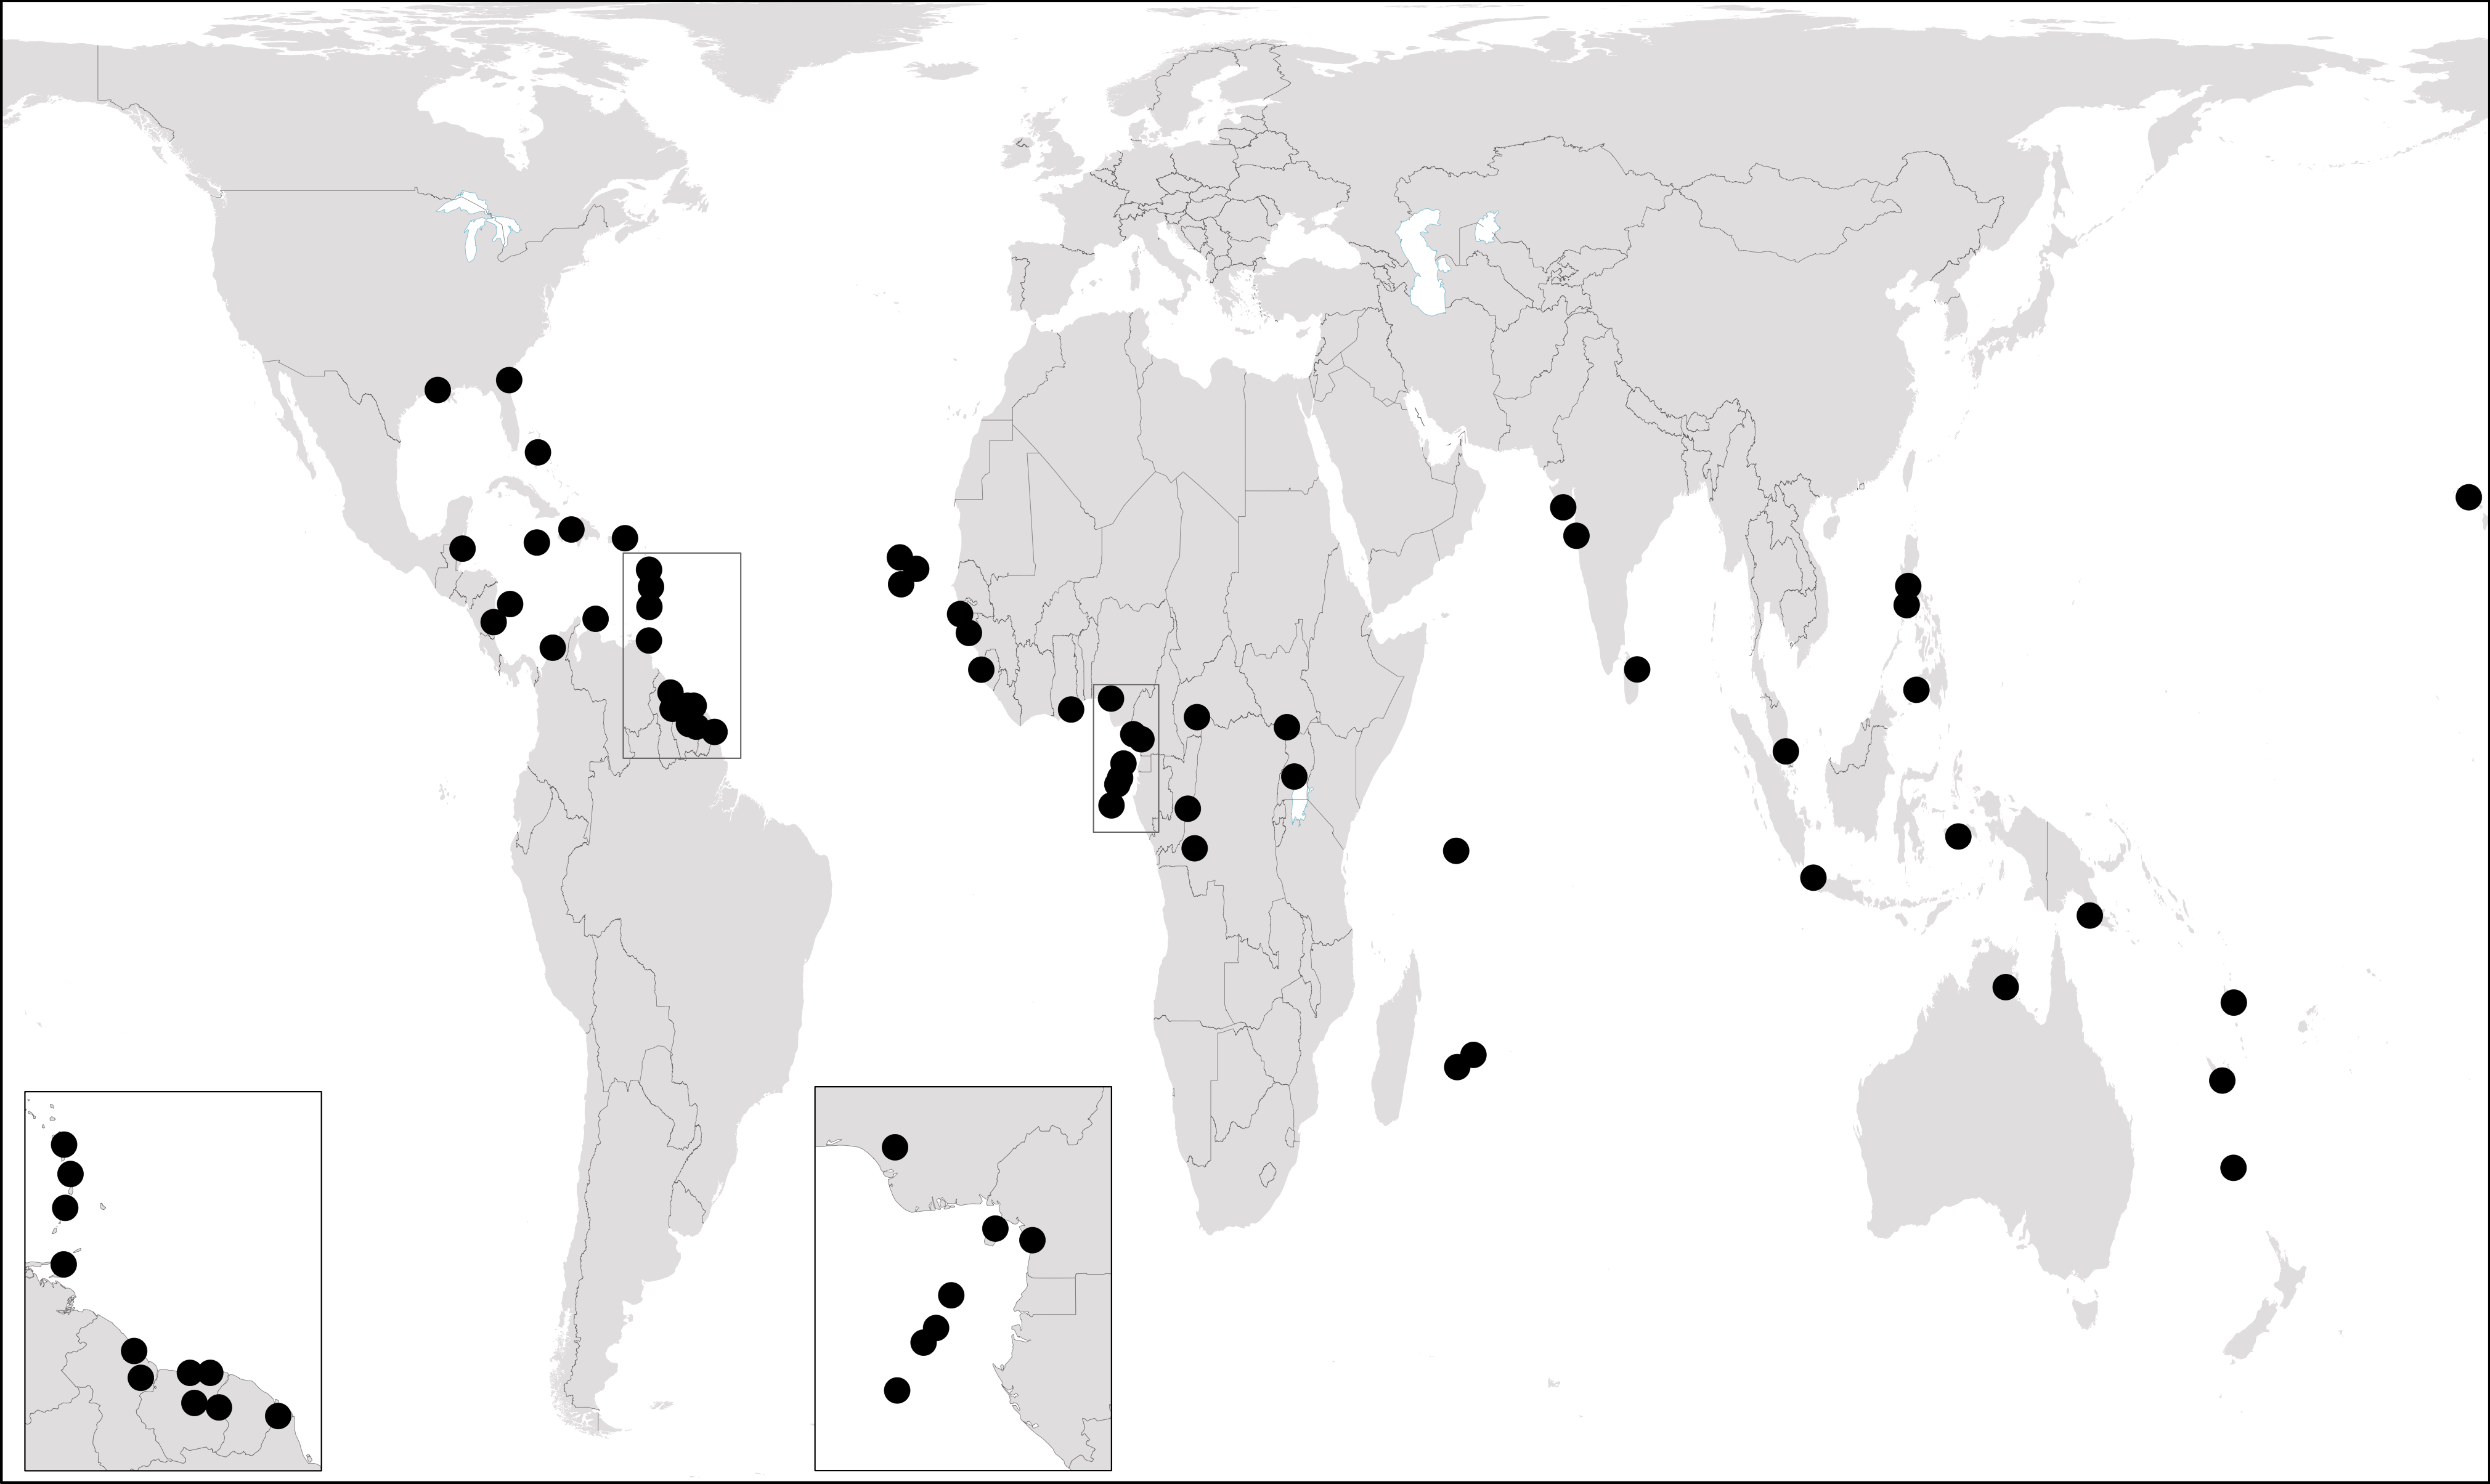
\includegraphics[width=\textwidth]{figures/Michaelis-Fig1.png}
\caption{Distribution of the 59 creole languages in \textit{APiCS} (for more information see apics-online.info) (CC BY-SA 4.0, Hans-Jörg Bibiko, MPI-SHH Jena)}
\label{fig:michaelis:1}
\end{figure}

\sloppy
\printbibliography[heading=subbibliography,notkeyword=this] 
\end{document}